
\chapter{Q-Learning}

% https://blog.csdn.net/qq_30615903/article/details/80739243
% https://www.freecodecamp.org/news/an-introduction-to-q-learning-reinforcement-learning-14ac0b4493cc/

% 视频 https://v.youku.com/v_show/id_XMTk2NzM1Mjk5Mg==.html

% 发现了很多RL资料搬砖过来,刚入门的可以用得上

% David Silver 博士的 UCL 公开课:http://www0.cs.ucl.ac.uk/staff/d.silver/web/Teaching.html
% DeepMind 和 UCL 的DL、RL课程:https://www.youtube.com/playlist?list=PLqYmG7hTraZDNJre23vqCGIVpfZ_K2RZs
% Sergey Levine 的DRL课程:http://rail.eecs.berkeley.edu/deeprlcourse/
% OpenAI 的 Spinning Up in Deep RL:https://blog.openai.com/spinning-up-in-deep-rl/
% 关于深度强化学习良心paper:https://arxiv.org/abs/1810.06339

In reinforcement learning, the state-value function is usually denoted by $v$, 
while the action-value function is denoted by $q$.
The $q$ in $q$-learning is in fact refer to the action-value function. 
$Q$-learning is at the heart of all reinforcement learning algorithms.

\section{What is $Q$-Learning ?}

$Q$-Learning is a Reinforcement learning policy that will find the next best action, 
given a current state. It chooses this action at random and aims to maximize the reward.

\begin{figure}[!htb]
\centering
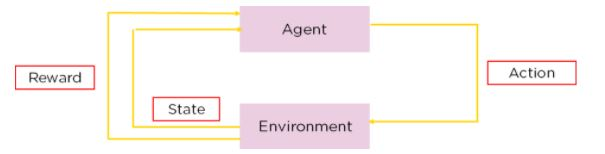
\includegraphics[scale=0.618]{pix/q_learning/3-components-q.jpg}
\caption{Components of Q-Learning}
%\label{fig:label}
\end{figure}

$Q$-learning is a model-free, off-policy reinforcement learning that will find the best 
course of action, given the current state of the agent. Depending on where the agent is 
in the environment, it will decide the next action to be taken.

Model-free means that the agent uses predictions of the environment's expected response 
to move forward. It does not use the reward system to learn, but rather, trial and error.

An example of $Q$-learning is an Advertisement recommendation system. In a normal ad 
recommendation system, the ads you get are based on your previous purchases or websites 
you may have visited. If you've bought a TV, you will get recommended TVs of different 
brands. 

\begin{figure}[!htb]
\centering

\includegraphics[scale=0.618]{pix/q_learning/4-adrecommend.jpg}
\caption{Ad Recommendation System}
%\label{fig:label}
\end{figure}

Using $Q$-learning, we can optimize the ad recommendation system to recommend products 
that are frequently bought together. The reward will be if the user clicks on the 
suggested product.

\begin{figure}[!htb]
\centering

\includegraphics[scale=0.618]{pix/q_learning/5-ad-q.jpg}
\caption{Ad Recommendation System with Q-Learning}
%\label{fig:label}
\end{figure}


\subsection{Important Terms in Q-Learning}

\begin{itemize}
%\setlength{\itemsep}{0pt}
%\setlength{\parsep}{0pt}
\setlength{\parskip}{0pt}
\item[1.]
States: The State, $S$, represents the current position of an agent in an environment.
\item[2.]
Action: The Action, $A$, is the step taken by the agent when it is in a particular state.
\item[3.]
Rewards: For every action, the agent will get a positive or negative reward.
\item[4.]
Episodes: When an agent ends up in a terminating state and can't take a new action.
\item[5.]
$Q$-Values: Used to determine how good an Action, $A$, taken at a particular state, $S$, 
is. $Q (A, S)$.
\item[6.]
Temporal Difference: A formula used to find the $Q$-Value by using the value of current 
state and action and previous state and action.
\end{itemize}


\subsection{What Is The Bellman Equation?}

The Bellman Equation is used to determine the value of a particular state and deduce 
how good it is to be in/take that state. The optimal state will give us the highest 
optimal value. 

The equation is given below. It uses the current state, and the reward associated with 
that state, along with the maximum expected reward and a discount rate, which determines 
its importance to the current state, to find the next state of our agent. The learning 
rate determines how fast or slow, the model will be learning. 

\begin{figure}[!htb]
\centering
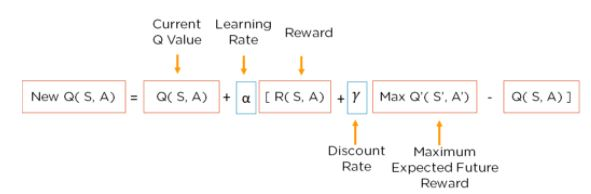
\includegraphics[scale=0.618]{pix/q_learning/6-bellman.jpg}
\caption{Bellman Equation}
%\label{fig:label}
\end{figure}


\subsection{A simplistic example}

Let's say that a robot has to cross a maze and reach the end point. There are mines, 
and the robot can only move one tile at a time. If the robot steps onto a mine, the 
robot is dead. The robot has to reach the end point in the shortest time possible.

The scoring/reward system is as below:
\begin{itemize}
%\setlength{\itemsep}{0pt}
%\setlength{\parsep}{0pt}
\setlength{\parskip}{0pt}
\item[1.]
The robot loses 1 point at each step. This is done so that the robot takes the 
shortest path and reaches the goal as fast as possible.

\item[2.]
If the robot steps on a mine, the point loss is 100 and the game ends.

\item[3.]
If the robot gets power \textcolor{magenta}{⚡️}, it gains 1 point.

\item[4.]
If the robot reaches the end goal, the robot gets 100 points.
\end{itemize}

Now, the obvious question is: {\bf How do we train a robot to reach the end goal 
with the shortest path without stepping on a mine?}

\begin{figure}[!htb]
\centering
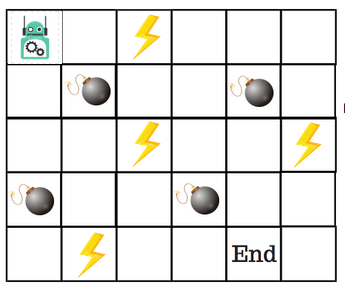
\includegraphics[scale=0.618]{pix/q_learning/q_robot_maze.png}
\caption{Maze}
%\label{fig:label}
\end{figure}
So, how do we solve this?


\subsection{Introducing the $Q$-Table}

\begin{tabular}{|c||c|c|}
\hline
$Q$-Table	& $a_1$	& $a_2$ \\
\hline
$s_1$	& $q(s_1,a_1)$	& $q(s_1,a_2)$ \\
\hline
$s_2$	& $q(s_2,a_1)$	& $q(s_2,a_2)$ \\
\hline
$s_3$	& $q(s_3,a_1)$	& $q(s_3,a_2)$ \\
\hline
\end{tabular}\;

\vspace

$Q$-Table is just a fancy name for a simple lookup table where we calculate the 
maximum expected future rewards for action at each state. Basically, this table 
will guide us to the best action at each state.

\begin{figure}[!htb]
\centering
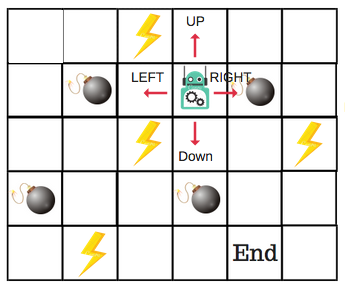
\includegraphics[scale=0.618]{pix/q_learning/q_robot_maze_actions.png}
\caption{Maze: actions}
%\label{fig:label}
\end{figure}
There will be four numbers of actions at each non-edge tile. When a robot is at a 
state it can either move up or down or right or left.

So, let's model this environment in our $Q$-Table.

In the $Q$-Table, the columns are the actions and the rows are the states.

\begin{figure}[!htb]
\centering
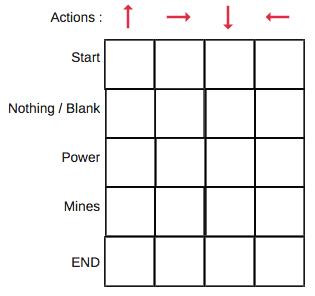
\includegraphics[scale=0.618]{pix/q_learning/q_robot_maze_table.png}
\caption{Maze: $q$-table}
%\label{fig:label}
\end{figure}

Each $Q$-table score will be the maximum expected future reward that the robot will 
get if it takes that action at that state. This is an iterative process, as we need 
to improve the $Q$-Table at each iteration.

But the questions are:

\begin{itemize}
%\setlength{\itemsep}{0pt}
%\setlength{\parsep}{0pt}
\setlength{\parskip}{0pt}
\item[-]
How do we calculate the values of the $Q$-table?
\item[-]
Are the values available or predefined?
\end{itemize}

To learn each value of the $Q$-table, we use the $Q$-Learning algorithm.


\subsection{How to Make a $Q$-Table?}

While running our algorithm, we will come across various solutions and the agent 
will take multiple paths. How do we find out the best among them? This is done by 
tabulating our findings in a table called a $Q$-Table.

A $Q$-Table helps us to find the best action for each state in the environment. We 
use the Bellman Equation at each state to get the expected future state and reward 
and save it in a table to compare with other states. 

Lets us create a $q$-table for an agent that has to learn to run, fetch and sit on 
command. The steps taken to construct a $q$-table are :

{\bf Step 1}: Create an initial $Q$-Table with all values initialized to $0$

When we initially start, the values of all states and rewards will be $0$. Consider 
the $Q$-Table shown below which shows a dog simulator learning to perform actions :

\begin{figure}[!htb]
\centering
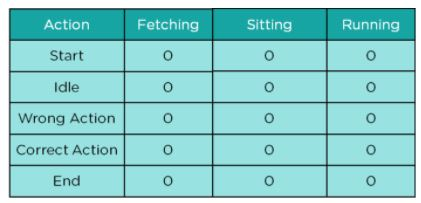
\includegraphics[scale=0.618]{pix/q_learning/7-initial.jpg}
\caption{Initial $q$-table}
%\label{fig:label}
\end{figure}

{\bf Step 2}: Choose an action and perform it. Update values in the $q$-table

This is the starting point. We have performed no other action as of yet. Let us say 
that we want the agent to sit initially, which it does. The table will change to:

\begin{figure}[!htb]
\centering
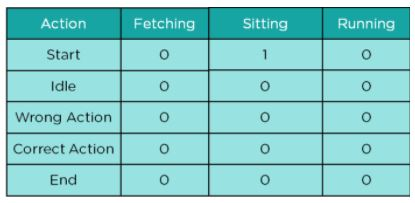
\includegraphics[scale=0.618]{pix/q_learning/8-qtable.jpg}
\caption{$Q$-table after performing an action}
%\label{fig:label}
\end{figure}

{\bf Step 3}: Get the value of the reward and calculate the value $Q$-Value using 
Bellman Equation

For the action performed, we need to calculate the value of the actual reward and 
the $Q( S, A )$ value

\begin{figure}[!htb]
\centering
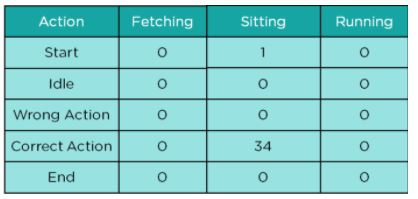
\includegraphics[scale=0.618]{pix/q_learning/9-updatingq.jpg}
\caption{Updating $q$-table with Bellman Equation}
%\label{fig:label}
\end{figure}

{\bf Step 4}: Continue the same until the table is filled or an episode ends

The agent continues taking actions and for each action, the reward and $Q$-value are 
calculated and it updates the table.

\begin{figure}[!htb]
\centering
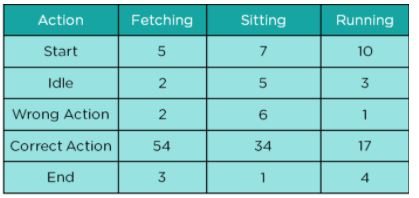
\includegraphics[scale=0.618]{pix/q_learning/10-finalq.jpg}
\caption{Final $q$-table at end of an episode}
%\label{fig:label}
\end{figure}


\section{Mathematics behind the Q-Learning algorithm}

\subsection{Q-function}

The Q-function uses the Bellman equation and takes two inputs: state (s) and action (a).

\begin{figure}[!htb]
\centering
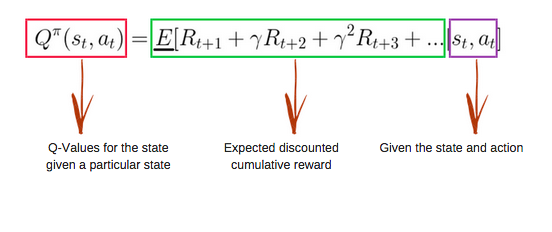
\includegraphics[scale=0.618]{pix/q_learning/q_function.png}
\caption{Maze: q-function}
%\label{fig:label}
\end{figure}

Using the above function, we get the values of Q for the cells in the table.

When we start, all the values in the Q-table are zeros.

There is an iterative process of updating the values. As we start to explore the 
environment, the Q-function gives us better and better approximations by continuously 
updating the Q-values in the table.

Now, let's understand how the updating takes place.


\subsection{Introducing the $Q$-learning algorithm process}

\begin{figure}[!htb]
\centering
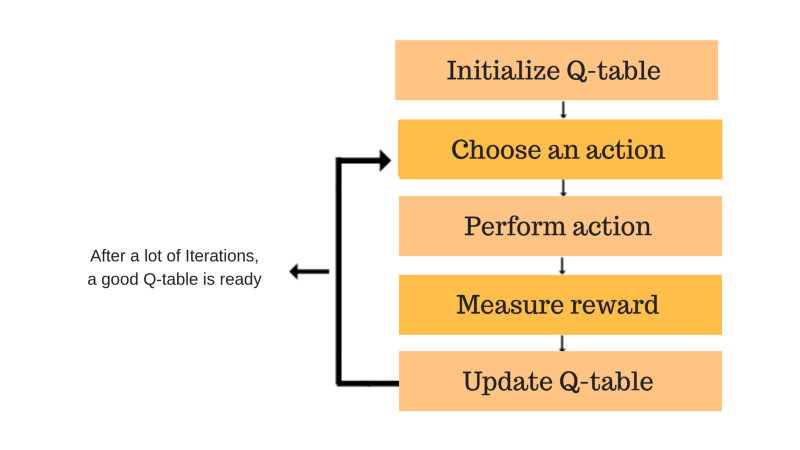
\includegraphics[scale=0.4]{pix/q_learning/q_learning_algorithm_process.png}
\caption{Maze: algorithm process}
%\label{fig:label}
\end{figure}
Each of the colored boxes is one step. Let's understand each of these steps in detail.


\subsubsection{Step 1: initialize the $Q$-Table}
We will first build a $Q$-table. There are $n$ columns, where $n=$ number of actions. 
There are m rows, where m= number of states. We will initialise the values at 0.

\begin{figure}[!htb]
\centering
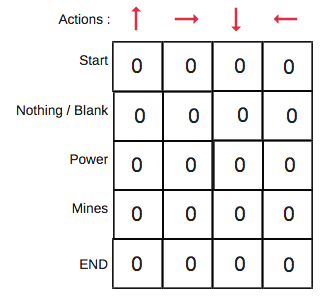
\includegraphics[scale=0.5]{pix/q_learning/q_robot_maze_table_init.png}
\caption{Maze: q-table initialization}
%\label{fig:label}
\end{figure}
In our robot example, we have four actions ($a=4$) and five states ($s=5$). So we will 
build a table with four columns and five rows.


\subsubsection{Steps 2 and 3: choose and perform an action}

This combination of steps is done for an undefined amount of time. This means that 
this step runs until the time we stop the training, or the training loop stops as 
defined in the code.

We will choose an action ($a$) in the state ($s$) based on the $Q$-Table. But, as 
mentioned earlier, when the episode initially starts, every $Q$-value is $0$.

So now the concept of exploration and exploitation trade-off comes into play. This 
chapter has more details.

We'll use something called the {\bf epsilon greedy strategy}.

In the beginning, the epsilon rates will be higher. The robot will explore the 
environment and randomly choose actions. The logic behind this is that the robot 
does not know anything about the environment.

As the robot explores the environment, the epsilon rate decreases and the robot 
starts to exploit the environment.

During the process of exploration, the robot progressively becomes more confident in 
estimating the $Q$-values.

For the robot example, there are four actions to choose from: up, down, left, and 
right. We are starting the training now — our robot knows nothing about the 
environment. So the robot chooses a random action, say right.

\begin{figure}[!htb]
\centering
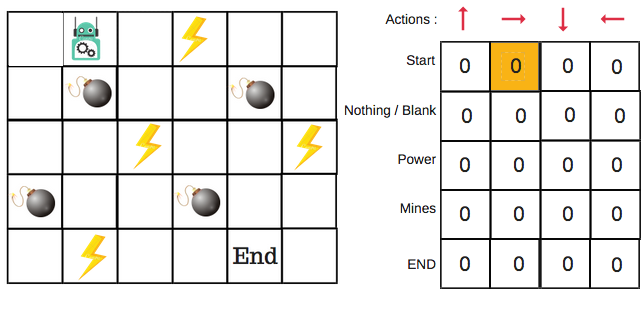
\includegraphics[scale=0.5]{pix/q_learning/q_robot_maze_perform_action.png}
\caption{Maze: perform an action}
%\label{fig:label}
\end{figure}

We can now update the $Q$-values for being at the start and moving right using the 
Bellman equation.


\subsubsection{Steps 4 and 5: evaluate}

Now we have taken an action and observed an outcome and reward. We need to update 
the function $Q(s,a)$.

\begin{figure}[!htb]
\centering
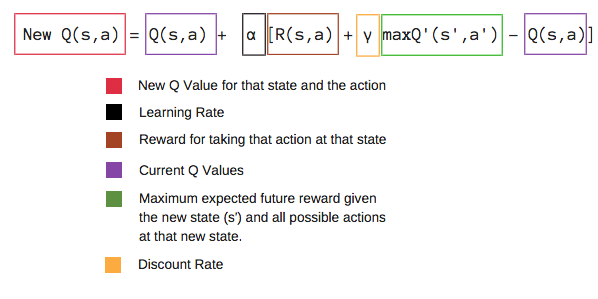
\includegraphics[scale=0.5]{pix/q_learning/q_robot_maze_q_function.png}
\caption{Maze: q-function}
%\label{fig:label}
\end{figure}

In the case of the robot game, to reiterate the scoring/reward structure is:

\begin{itemize}
%\setlength{\itemsep}{0pt}
%\setlength{\parsep}{0pt}
\setlength{\parskip}{0pt}
\item[-]
power $= +1$
\item[-]
mine $= -100$
\item[-]
end $= +100$
\end{itemize}

\begin{figure}[!htb]
\centering
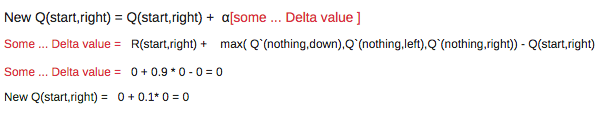
\includegraphics[scale=0.7]{pix/q_learning/q_robot_maze_iteration.png}
%\caption{Maze: q-function}
%\label{fig:label}
\end{figure}
We will repeat this again and again until the learning is stopped. In this way 
the $Q$-Table will be updated.


\section{Implementation using python}
\begin{lstlisting}[language=Python]
\end{lstlisting}

Let's use $Q$-Learning to find the shortest path between two points. We have a group 
of nodes and we want the model to automatically find the shortest way to travel from 
one node to another. We start by importing the necessary modules:

\begin{lstlisting}[language=Python]
import numpy as np
\end{lstlisting}

Then we define all possible actions or the points/nodes that exist.
\begin{lstlisting}[language=Python]
# Define the actions
actions = [0,1,2,3,4,5,6,7,8]
\end{lstlisting}

We define the rewards array for every action.
\begin{lstlisting}[language=Python]
# Define the rewards
rewards = np.array([[0,1,0,0,0,0,0,0,0],
[1,0,1,0,1,0,0,0,0],
[0,1,0,0,0,1,0,0,0],
[0,0,0,0,0,0,1,0,0],
[0,1,0,0,0,0,0,1,0],
[0,0,1,0,0,0,0,0,0],
[0,0,0,1,0,0,0,1,0],
[0,0,0,0,1,0,1,0,1],
[0,0,0,0,0,0,0,1,0]])
\end{lstlisting}

% https://www.simplilearn.com/tutorials/machine-learning-tutorial/what-is-q-learning


\subsection{公式推导}

% https://blog.csdn.net/qq_30615903/article/details/80739243

举个例子如图有一个 GridWorld 的游戏从起点出发到达终点为胜利掉进陷阱为失败。智能体(Agent)、
环境状态(environment)、奖励(reward)、动作(action)可以将问题抽象成一个马尔科夫决策过程,
我们在每个格子都算是一个状态 $s_t$, $\pi(a|s)$ 在 $s$ 状态下采取动作 $a$ 策略 。 
$P(s'|s,a)$ 也可以写成 $P_{ss'}^a$ 为在 $s$ 状态下选择 $a$ 动作转换到下一个状态 $s'$ 的概率。
$R(s'|s,a)$ 表示在 $s$ 状态下采取 $a$ 动作转移到 $s'$ 的奖励 reward,
我们的目的很明确就是找到一条能够到达终点获得最大奖赏的策略。

An agent is in the bottom left cell of a grid. The grey cell is a wall. The two coloured 
cells give a reward. There is a reward of $1$ of being in the top-right (diamond) cell, 
but a negative value of $-1$ for the cell immediately below (explosive).

\begin{figure}[!htb]
\centering
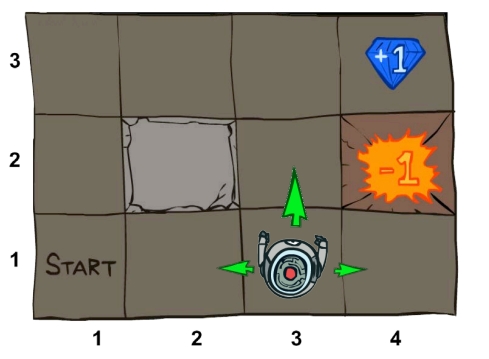
\includegraphics[scale=0.7]{pix/q_learning/gridworld.png}
%\caption{Example: Gridworld}
%\label{fig:label}
\end{figure}

问题模型 -- An MDP defined by:
\begin{itemize}
%\setlength{\itemsep}{0pt}
%\setlength{\parsep}{0pt}
\setlength{\parskip}{0pt}
\item[-]
Set of states $\mathcal{S}$

\item[-]
Set of actions $\mathcal{A}$

\item[-]
Transition function $P(s'|s, a)$

\item[-]
Reward function $R(s,a,s')$

\item[-]
Start state $s_0$

\item[-]
Discount factor $\gamma$

\item[-]
Horizon $H$

\end{itemize}


目标:找到使得累计奖励期望值最大的策略
$$
\max_\pi E\left[ \sum_{t=0}^H \gamma^t R(S_t, A_t, S_{t+1}) | \pi \right]
$$

$Q$-learning 的主要优势就是使用了时间差分法TD(融合了蒙特卡洛和动态规划)能够进行离线学习, 
使用 Bellman 方程可以对马尔科夫过程求解最优策略。






